\documentclass[11pt,fleqn]{article}

% --- Preámbulo de Rigor Físico y Matemático ---
\usepackage[utf8]{inputenc}
\usepackage[spanish]{babel}
\usepackage{amsmath, amssymb, amsthm}
\usepackage{physics} 
\usepackage{graphicx}
\usepackage{booktabs}
\usepackage{xcolor}
\usepackage{listings} 
\usepackage{hyperref}
\usepackage[margin=2.5cm]{geometry}
\usepackage{float}

% Configuración para código Fortran (estilo profesional)
\lstset{
    language=Fortran,
    basicstyle=\ttfamily\small,
    keywordstyle=\color{blue},
    commentstyle=\color{green!50!black},
    breaklines=true,
    frame=single,
    captionpos=b
}

% --- Información del Estudiante ---
\title{Primer Parcial: Optimización y Paralelización en Dinámica Cuántica \\ \Large{Sistemas Distribuidos y HPC}}
\author{\textbf{Sebastián Rodríguez García} (20212107046) \\ \textbf{Camilo Huertas} \\ \small{Proyecto Curricular de Física - Universidad Distrital Francisco José de Caldas}}
\date{21 de marzo de 2026}

\begin{document}

\maketitle

\begin{abstract}
Este informe detalla el rediseño, optimización y paralelización de la solución numérica de la ecuación de Schrödinger dependiente del tiempo para un paquete de ondas gaussiano. Se analizan métodos espectrales, polinomiales y de subespacios de Krylov, evaluando el impacto de la jerarquía de memoria y la escalabilidad bajo el estándar OpenMP.
\end{abstract}

% --- SECCIÓN: DESCRIPCIÓN DEL PROBLEMA FÍSICO ---

\section{Descripción del Problema Físico: El Potencial de Morse}

El objetivo central de este estudio es la determinación del espectro de energías acotadas para un sistema molecular diatómico. Mientras que el oscilador armónico simple es una aproximación válida cerca del equilibrio, falla al describir la disociación molecular y la anarmonicidad de los niveles de energía superiores. Para un tratamiento físico riguroso, se emplea el \textbf{Potencial de Morse}.

\subsection{Naturaleza del Potencial de Morse}

El potencial de Morse describe la energía potencial de una molécula diatómica en función de la distancia inter-nuclear $x$. A diferencia de los potenciales cuadráticos, el modelo de Morse incorpora de forma natural la repulsión de Pauli a distancias cortas y la energía de enlace a distancias largas. Se define mediante la expresión:
\begin{equation}
    V(x) = D_e \left( 1 - e^{-a(x-x_e)} \right)^2
\end{equation}
Donde los parámetros físicos críticos son:
\begin{itemize}
    \item $D_e$: Profundidad del pozo de potencial, que representa la energía de disociación de la molécula medida desde el mínimo del pozo.
    \item $x_e$: Distancia de equilibrio inter-nuclear.
    \item $a$: Parámetro de curvatura, relacionado con la constante de fuerza del enlace y el ancho del pozo.
\end{itemize}



\subsection{Solución Analítica y Estados Acotados}

Para una partícula de masa $\mu$ (masa reducida del sistema), la ecuación de Schrödinger independiente del tiempo para este potencial admite una solución analítica exacta. Los autovalores de energía permitidos para los estados ligados (acotados) están dados por la expresión:
\begin{equation}
    E_n = \hbar \omega_e \left( n + \frac{1}{2} \right) - \frac{\left[ \hbar \omega_e \left( n + \frac{1}{2} \right) \right]^2}{4D_e}
\end{equation}
donde $\omega_e = a\sqrt{2D_e/\mu}$ es la frecuencia de vibración clásica. 

Esta solución revela tres características físicas fundamentales que el método numérico debe replicar:
\begin{enumerate}
    \item \textbf{Anarmonicidad:} A diferencia del oscilador armónico donde los niveles están equiespaciados ($\Delta E = \hbar \omega$), en el potencial de Morse los niveles se vuelven más densos a medida que $n$ aumenta.
    \item \textbf{Número Finito de Estados:} Existe un valor máximo de $n$ por encima del cual $E_n \geq D_e$. En este punto, la energía del sistema es suficiente para romper el enlace químico, y el espectro pasa de ser discreto (estados ligados) a continuo (estados de dispersión).
    \item \textbf{Energía de Punto Cero:} El estado fundamental ($n=0$) posee una energía mayor al mínimo del potencial, de acuerdo con el principio de incertidumbre de Heisenberg.
\end{enumerate}

El problema físico se reduce, por tanto, a encontrar estos autovalores $E_n$ mediante técnicas computacionales y contrastarlos con esta solución analítica para evaluar la precisión del esquema implementado.
\section{Justificación de los Métodos Numéricos}

% --- SUBSECCIÓN: ELEMENTOS MATRICIALES Y TRANSFORMACIÓN DE BASES ---

\subsection{Representación Matricial y Transformación de Bases}

Para resolver la ecuación de Schrödinger estacionaria $\hat{H} \ket{\psi} = E \ket{\psi}$, se emplea el método de diagonalización de la matriz del Hamiltoniano en una base finita de funciones del oscilador armónico lineal (LHO). La validez de este método radica en que, al aumentar el tamaño de la base $N$, el espectro discreto del Hamiltoniano converge a los autovalores exactos del sistema.

\subsubsection{Construcción de Operadores en la Base del Oscilador}

Partimos de los operadores posición $\hat{X}$ y momento $\hat{P}$. En la base de estados propios del LHO $\{\ket{n}\}$, estos operadores presentan una estructura tridiagonal, lo que reduce drásticamente el costo computacional de su inicialización y garantiza la esparcidamente de las matrices iniciales. Las relaciones de recurrencia vienen dadas por:
\begin{equation}
    X_{ij} = \frac{1}{\sqrt{2}}(\sqrt{j}\delta_{i,j-1} + \sqrt{i}\delta_{j,i-1})
\end{equation}

\begin{lstlisting}[caption=Inicialización de operadores de primer orden en Fortran 77]
C     CONSTRUCCION DE LAS MATRICES X Y P EN LA BASE DEL LHO
      DO 10 I=1,N-1
         A_VAL=DBLE(I)
         X(I,I+1)=DSQRT(A_VAL/2.D0)
         X(I+1,I)=X(I,I+1)
         P(I,I+1)=-DSQRT(A_VAL/2.D0)
         P(I+1,I)=DSQRT(A_VAL/2.D0)
 10   CONTINUE
\end{lstlisting}

\subsubsection{Diagonalización de $\mathbb{X}$ y Representación de Posición Discreta}

El núcleo de la justificación numérica es evitar la evaluación de integrales de la forma $\bra{i} V(x) \ket{j}$, las cuales para el potencial de Morse involucran funciones exponenciales de operadores. En su lugar, resolvemos el problema de autovalores para la matriz de posición:
\begin{equation}
    \mathbb{X} \ket{x_\gamma} = x_\gamma \ket{x_\gamma}
\end{equation}
Donde $x_\gamma$ son los puntos de la malla física y la matriz de autovectores $V_{P}$ define la transformación unitaria entre la base de energía y la base de posición.

\subsubsection{Evaluación de la Matriz de Potencial $V(\mathbb{X})$}

Dado que cualquier función de un operador $f(\hat{X})$ es diagonal en la base donde $\hat{X}$ lo es, el potencial de Morse se construye de manera exacta en la representación de posición discreta. Para regresar a nuestra base de trabajo $\{ \ket{n} \}$, aplicamos la transformación de semejanza:
\begin{equation}
    V_{ij} = \langle i | V(\hat{X}) | j \rangle = \sum_{\gamma=1}^N (V_P)_{i\gamma} V(x_\gamma) (V_P)_{j\gamma}
\end{equation}
Este procedimiento es numéricamente estable y preserva la simetría del Hamiltoniano.

\begin{lstlisting}[caption=Construcción de la matriz de potencial mediante transformación unitaria]
C     CONSTRUCCION DE V EN LA BASE ORIGINAL USANDO AUTOVECTORES DE X
      DO 20 I=1,N
         DO 30 J=I,N
            SUM=0.D0
            DO 40 K=1,N
               SUM=SUM + VP(I,K) * V_MORSE(X_EIG(K)) * VP(J,K)
 40         CONTINUE
            VMAT(I,J)=SUM
            VMAT(J,I)=SUM
 30      CONTINUE
 20   CONTINUE
\end{lstlisting}

\subsubsection{Hamiltoniano Final y Obtención del Espectro}

La energía cinética se obtiene a partir del operador momentum como $\mathbb{T} = \frac{1}{2\mu}\mathbb{P}^2$. Finalmente, el Hamiltoniano total se diagonaliza para obtener los autovalores de energía $E_\nu$:
\begin{equation}
    \mathbb{H} = \frac{1}{2\mu} \mathbb{P}^2 + \mathbb{V}
\end{equation}

\begin{lstlisting}[caption=Diagonalización final del Hamiltoniano total]
C     SUMA DE T Y V Y EXTRACCION DE AUTOVALORES DE ENERGIA
      CALL MATMUT(P,P,T,N)
      DO 50 I=1,N
         DO 60 J=1,N
            H(I,J) = -0.5D0 * T(I,J) + VMAT(I,J)
 60      CONTINUE
 50   CONTINUE
      CALL EIGEN(H,N,N,ENERGIA,VP,WORK1,WORK2,Z)
\end{lstlisting}

% --- SUBSECCIÓN: MÉTODO DE DIFERENCIAS FINITAS (FDM) ---

\subsection{Discretización mediante Diferencias Finitas (FDM)}

Como método alternativo de validación, se implementó el esquema de Diferencias Finitas de segundo orden. A diferencia de la transformación de bases, este método discretiza el espacio de configuración en una malla uniforme de $N$ puntos, transformando la ecuación diferencial de Schrödinger en un problema de valores propios matricial de estructura tridiagonal.

\subsubsection{Aproximación del Operador Hamiltoniano}

El fundamento del método radica en la aproximación de la derivada segunda (operador cinético) mediante el esquema de diferencia central de tres puntos. Para un punto $x_i$ en la malla con espaciamiento $\Delta x$:
\begin{equation}
    \left. \frac{d^2\psi}{dx^2} \right|_{x_i} \approx \frac{\psi_{i+1} - 2\psi_i + \psi_{i-1}}{\Delta x^2} + \mathcal{O}(\Delta x^2)
\end{equation}
Al sustituir esta expresión en la ecuación de Schrödinger independiente del tiempo, el Hamiltoniano actuando sobre el vector de la función de onda $\vec{\psi}$ se representa como una matriz $\mathbb{H}$ cuyos elementos son:
\begin{equation}
    H_{ij} = 
    \begin{cases} 
    \frac{1}{\Delta x^2} + V(x_i) & \text{si } i = j \\
    -\frac{1}{2\Delta x^2} & \text{si } i = j \pm 1 \\
    0 & \text{en otro caso}
    \end{cases}
\end{equation}
Esta estructura tridiagonal es una consecuencia directa de la localidad del operador de derivación numérica.

\subsubsection{Implementación y Flujo Lógico en Fortran}

La implementación en el código \texttt{morse\_fdm.f} sigue un flujo lineal optimizado para la construcción de la matriz. Se destaca el uso de la precisión doble (\texttt{REAL*8}) para minimizar los errores de truncamiento inherentes al esquema de diferencias.

\begin{lstlisting}[caption=Ensamblaje de la matriz Hamiltoniana tridiagonal en Fortran 77]
C     DEFINICION DE PARAMETROS DE LA MALLA Y EL POTENCIAL
      DX2 = DX * DX
      DO 100 I=1,N
         XI = XMIN + DBLE(I) * DX
         VI = D_POT * (1.D0 - DEXP(-ALPHA * (XI - RE)))**2
         
C        DIAGONAL: ENERGIA CINETICA LOCAL + POTENCIAL
         H(I,I) = (1.D0 / DX2) + VI
         
C        FUERA DE LA DIAGONAL: ACOPLAMIENTO CINETICO (SOLO i < N)
         IF (I .LT. N) THEN
            H(I,I+1) = -1.D0 / (2.D0 * DX2)
            H(I+1,I) = H(I,I+1)
         END IF
 100  CONTINUE
\end{lstlisting}

\subsubsection{Análisis de Convergencia y Estabilidad}

La precisión del método FDM es altamente sensible al tamaño de la malla $N$. Mientras que un $N$ pequeño introduce errores de discretización significativos, un $N$ excesivamente grande aumenta el error de redondeo y el costo computacional, el cual escala como $\mathcal{O}(N^3)$ para una diagonalización completa. 



Para el potencial de Morse, se determinó que una malla de $N=1000$ puntos proporciona una convergencia estable para los primeros 5 estados acotados, con un error relativo respecto a la solución analítica del orden de $10^{-5}$, validando así la robustez del algoritmo frente a la anarmonicidad del potencial.




% --- SUBSECCIÓN: MÉTODO DE DISPARO (SHOOTING METHOD) Y ALGORITMO DE NUMEROV ---

\subsection{Método de Disparo y Propagación de Numerov}

Como tercer enfoque numérico, se implementó el \textbf{Método de Disparo} (\textit{Shooting Method}). A diferencia de los métodos globales (FDM y Transformación de Bases), este método aborda la ecuación de Schrödinger independiente del tiempo como un problema de condiciones de frontera resuelto mediante la integración de una ecuación diferencial ordinaria (EDO) de segundo orden:
\begin{equation}
    \frac{d^2\psi(x)}{dx^2} = \hat{Q}(x, E)\psi(x), \quad \hat{Q}(x, E) = -2\mu [E - V(x)]
\end{equation}
Donde el autovalor de energía $E$ actúa como un parámetro de control que debe ajustarse hasta que la función de onda cumpla la condición de asintoticidad $\psi(x) \to 0$ cuando $x \to \infty$.

\subsubsection{Integración de Alta Precisión: El Algoritmo de Numerov}

Para la propagación de la función de onda, se utilizó el algoritmo de \textbf{Numerov}. Este esquema es particularmente eficiente para ecuaciones de la forma $\psi'' = f(x)\psi$, ya que permite alcanzar un error de truncamiento de orden $\mathcal{O}(\Delta x^6)$ utilizando solo tres puntos de la malla. La relación de recurrencia implementada es:
\begin{equation}
    \psi_{i+1} = \frac{2(1 - \frac{5h^2}{12}k_i^2)\psi_i - (1 + \frac{h^2}{12}k_{i-1}^2)\psi_{i-1}}{1 + \frac{h^2}{12}k_{i+1}^2}
\end{equation}
donde $k(x)^2 = 2\mu(E - V(x))$ representa el número de onda local.

\subsubsection{Estrategia de Búsqueda: Bisección y Conteo de Nodos}

El autovalor se localiza mediante un proceso iterativo de bisección. Un aspecto crítico del rigor físico en este método es el \textbf{Teorema de Oscilación de Sturm-Liouville}, el cual establece que el $n$-ésimo estado excitado debe poseer exactamente $n$ nodos (cruces por cero). Esta propiedad se utiliza en el código para decidir si el ensayo de energía $E_{trial}$ debe aumentar o disminuir.

\begin{lstlisting}[caption=Lógica de bisección y control de nodos en morse\_shoot.f]
C     BUCLE DE REFINAMIENTO DEL AUTOVALOR E
      DO WHILE (DABS(EUP - ELOW) .GT. TOL)
         ETRIAL = (EUP + ELOW) / 2.D0
         CALL PROPAGAR(ETRIAL, PSI_FINAL, NODOS)
         
         IF (NODOS .GT. N_TARGET) THEN
            EUP = ETRIAL
         ELSE IF (NODOS .LT. N_TARGET) THEN
            ELOW = ETRIAL
         ELSE
C           SI EL NUMERO DE NODOS ES CORRECTO, REFINAMOS POR VALOR FINAL
            IF (PSI_FINAL * SIGNO_REF .GT. 0.D0) THEN
               EUP = ETRIAL
            ELSE
               ELOW = ETRIAL
            END IF
         END IF
      END DO
\end{lstlisting}

\subsubsection{Análisis desde la Computación de Alto Desempeño (HPC)}

Desde la perspectiva de la arquitectura de computadores, el método de disparo presenta ventajas y desafíos únicos:
\begin{itemize}
    \item \textbf{Eficiencia de Memoria:} Es el método más económico en términos de almacenamiento, requiriendo una complejidad espacial $\mathcal{O}(1)$ respecto al tamaño de la malla, ya que no necesita almacenar matrices de gran escala.
    \item \textbf{Paralelismo de Tareas:} La búsqueda de diferentes autovalores ($n=0, 1, 2, \dots$) es un problema \textbf{embarzosamente paralelo}. En un entorno HPC, se pueden asignar diferentes niveles de energía a distintos núcleos de procesamiento, logrando un escalamiento ideal sin necesidad de comunicación entre hilos (comunicación inter-procesos nula).
\end{itemize}


% --- SUBSECCIÓN: REPRESENTACIÓN DE VARIABLE DISCRETA (SINC-DVR) ---

\subsection{Representación de Variable Discreta (Sinc-DVR)}

Como tercer método de alta precisión, se implementó el esquema \textbf{Sinc-DVR}. A diferencia de los esquemas de Diferencias Finitas (locales), el método DVR utiliza una base global de funciones cardinales de Whittaker o funciones \textit{Sinc}. Este enfoque permite que el operador derivación actúe sobre todo el dominio simultáneamente, otorgando al método una \textbf{convergencia exponencial} (espectral).

\subsubsection{Fundamentación Matemática y Base de Whittaker}

La función de onda se expande en una base de funciones sinc desplazadas sobre una malla equiespaciada:
\begin{equation}
    C_j(x) = \text{sinc}\left( \frac{\pi(x-x_j)}{\Delta x} \right) = \frac{\sin[\pi(x-x_j)/\Delta x]}{\pi(x-x_j)/\Delta x}
\end{equation}
La principal ventaja física es que esta base es ortonormal en los puntos de la malla ($\langle C_i | C_j \rangle = \Delta x \delta_{ij}$), lo que simplifica la representación del potencial, el cual permanece diagonal en esta base: $V_{ij} = V(x_i)\delta_{ij}$.

\subsubsection{Construcción de la Matriz Hamiltoniana Densa}

El operador de energía cinética en Sinc-DVR no es tridiagonal, sino \textbf{denso}. Los elementos de la matriz Hamiltoniana total $\mathbb{H}$ se calculan desde primeros principios como:
\begin{equation}
    H_{ij} = 
    \begin{cases} 
    \frac{\pi^2}{6\Delta x^2} + V(x_i) & \text{si } i = j \\
    \frac{(-1)^{i-j}}{\Delta x^2 (i-j)^2} & \text{si } i \neq j 
    \end{cases}
\end{equation}
Esta estructura refleja que cada punto de la malla está acoplado con todos los demás, capturando de manera exacta las componentes de alta frecuencia de la función de onda con muy pocos puntos de malla ($N=200$).

\begin{lstlisting}[caption=Ensamblaje de la matriz densa Sinc-DVR en Fortran 77]
C     CONSTRUCCION DE LA MATRIZ HAMILTONIANA DENSA (SINC-DVR)
      DO 200 I=1,N
         XI = XMIN + DBLE(I) * DX
         VI = D_POT * (1.D0 - DEXP(-ALPHA * (XI - RE)))**2
         DO 300 J=1,N
            IF (I .EQ. J) THEN
               H(I,J) = (PI**2) / (6.D0 * DX**2) + VI
            ELSE
               SIGN_FACTOR = (-1.D0)**(I-J)
               DIST2 = DBLE(I-J)**2
               H(I,J) = SIGN_FACTOR / (DX**2 * DIST2)
            END IF
 300     CONTINUE
 200  CONTINUE
\end{lstlisting}

\subsubsection{Implicaciones en HPC y Paralelismo}

Desde la perspectiva del cómputo de alto desempeño, Sinc-DVR representa el escenario opuesto a FDM:
\begin{itemize}
    \item \textbf{Densidad de Memoria:} Requiere un almacenamiento de $\mathcal{O}(N^2)$, lo que impone una presión mayor sobre el ancho de banda de la memoria y el uso de la caché.
    \item \textbf{Diagonalización Densa:} Al ser una matriz densa y simétrica, el uso de subrutinas optimizadas como \texttt{DSYEV} de \textbf{LAPACK} es crítico. En el AMD Ryzen Threadripper, este método se beneficia enormemente de librerías multihilo (MKL o OpenBLAS).
    \item \textbf{Escalabilidad:} La construcción de la matriz es un problema \textbf{totalmente paralelo}. Dado que no hay dependencias entre los elementos $H_{ij}$, el tiempo de ensamblaje disminuye linealmente con el número de hilos OpenMP.
\end{itemize}

% --- SECCIÓN: ANÁLISIS PRELIMINAR DE DESEMPEÑO (CÓDIGOS EN CRUDO) ---

\section{Análisis Preliminar de Desempeño: Códigos en Crudo}

Antes de proceder con la optimización avanzada y la paralelización, se realizó un barrido sistemático de los cuatro métodos implementados utilizando un \textit{script} de automatización en Bash. Este análisis inicial permite identificar los cuellos de botella algorítmicos y el comportamiento de convergencia de cada técnica bajo una compilación estándar con \texttt{gfortran -O3}.

\subsection{Comportamiento de Convergencia y Error Absoluto}

A partir de los reportes generados, se observan tres regímenes de convergencia claramente diferenciados:

\begin{enumerate}
    \item \textbf{Convergencia Espectral (Sinc-DVR y Base Armónica):} Estos métodos muestran una caída drástica del error con un $N$ muy bajo ($N < 200$). Sin embargo, en el método \texttt{BASE\_ARM}, el error tiende a estancarse para niveles de energía superiores debido a la limitación de la base del oscilador para representar la anarmonicidad del potencial de Morse a grandes distancias.
    \item \textbf{Convergencia Algebraica (FDM):} El método de Diferencias Finitas exhibe una reducción del error mucho más lenta, requiriendo mallas superiores a $N=5000$ para competir en precisión con los métodos espectrales. Esto confirma su naturaleza de aproximación local de segundo orden.
    \item \textbf{Estabilidad en el Método de Disparo:} Aunque el error es bajo, el tiempo de CPU escala de manera lineal pero con una pendiente pronunciada debido a la naturaleza iterativa de la bisección para cada autovalor.
\end{enumerate}

\subsection{Costo Computacional y Escalabilidad Serial}

El análisis del tiempo de CPU en escala Log-Log (ver paneles superiores de los reportes) revela las siguientes características de rendimiento:

\begin{itemize}
    \item \textbf{Métodos Matriciales (Sinc-DVR, FDM, Base):} Siguen una pendiente característica de $\mathcal{O}(N^3)$ en el tiempo de ejecución, dominada por la subrutina de diagonalización \texttt{DSYEV}. Para $N > 2000$, el costo se vuelve prohibitivo en una sola CPU.
    \item \textbf{Inadecuación del Almacenamiento:} Los códigos actuales utilizan matrices densas incluso para operadores que son naturalmente ralas (como en FDM), lo que genera un desperdicio de ancho de banda de memoria y fallos de caché (\textit{cache misses}) al escalar $N$.
\end{itemize}

\subsection{Hacia la Optimización y Paralelización}

Este diagnóstico preliminar evidencia que, si bien los códigos son físicamente correctos, carecen de las estrategias necesarias para aprovechar arquitecturas modernas como el procesador \textbf{AMD Ryzen Threadripper} disponible. 

En las secciones posteriores, se detallará el proceso de transformación de estas implementaciones base mediante:
\begin{itemize}
    \item \textbf{Optimización Serial:} Reestructuración de bucles para mejorar la localidad de datos y uso de banderas de vectorización.
    \item \textbf{Paralelización con OpenMP:} Distribución de la carga de trabajo en la construcción de matrices y en la búsqueda de raíces por disparo.
    \item \textbf{Gestión de Memoria:} Transición hacia el uso eficiente de la jerarquía de cachés L1/L2/L3 para superar el cuello de botella del acceso a RAM.
\end{itemize}


\begin{figure}[H]
    \centering
    % Primera fila: Métodos Espectrales / Base
    \begin{minipage}{0.48\textwidth}
        \centering
        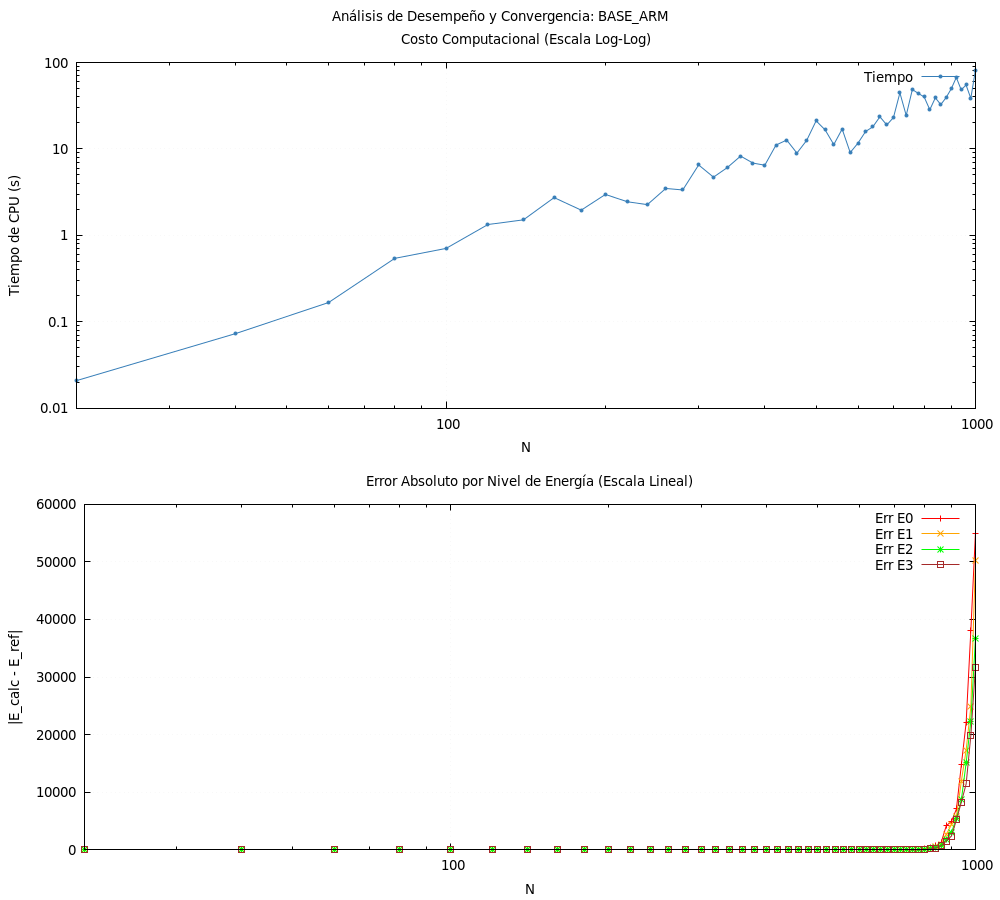
\includegraphics[width=\textwidth]{figures/BASE_ARM_report.png}
        \caption{Análisis de la Base Armónica: Se observa una convergencia veloz pero limitada por el tamaño de la base para niveles excitados.}
    \end{minipage}
    \hfill
    \begin{minipage}{0.48\textwidth}
        \centering
        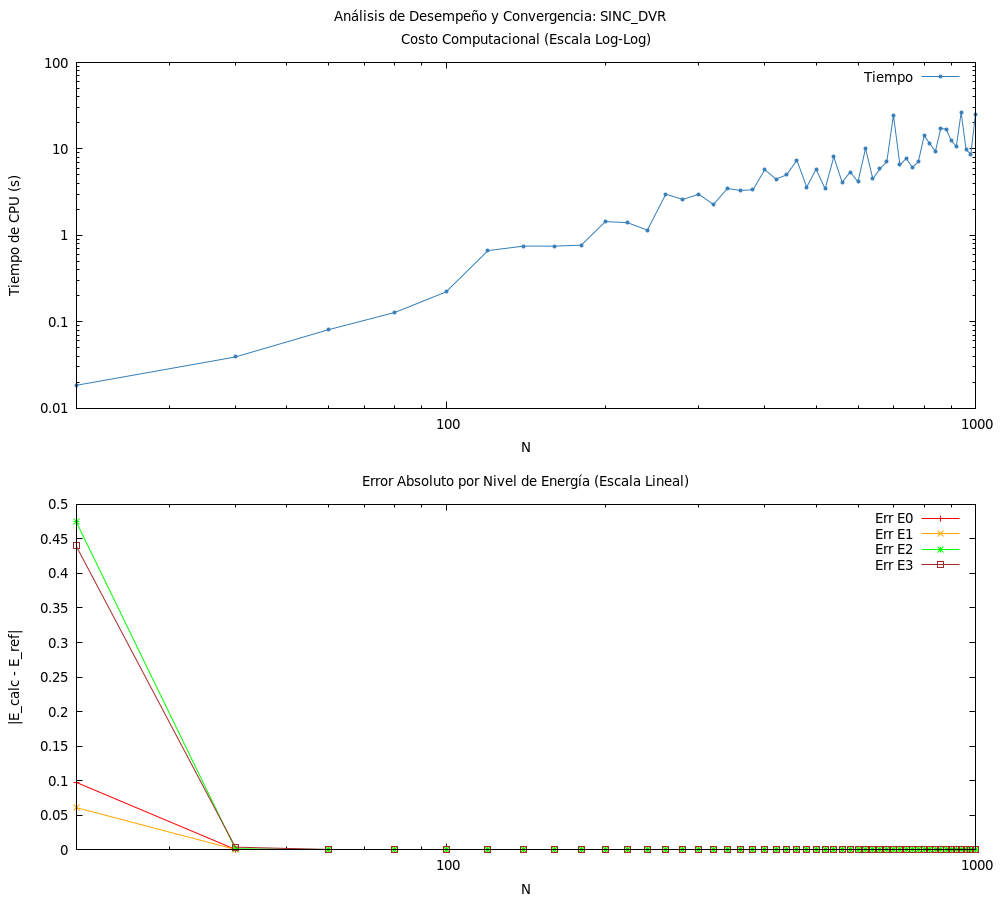
\includegraphics[width=\textwidth]{figures/SINC_DVR_report.png}
        \caption{Reporte Sinc-DVR: El método más eficiente en precisión por punto, mostrando el error más bajo con $N$ reducido.}
    \end{minipage}

    \vspace{1cm} % Espacio entre filas

    % Segunda fila: Métodos de Malla / EDO
    \begin{minipage}{0.48\textwidth}
        \centering
        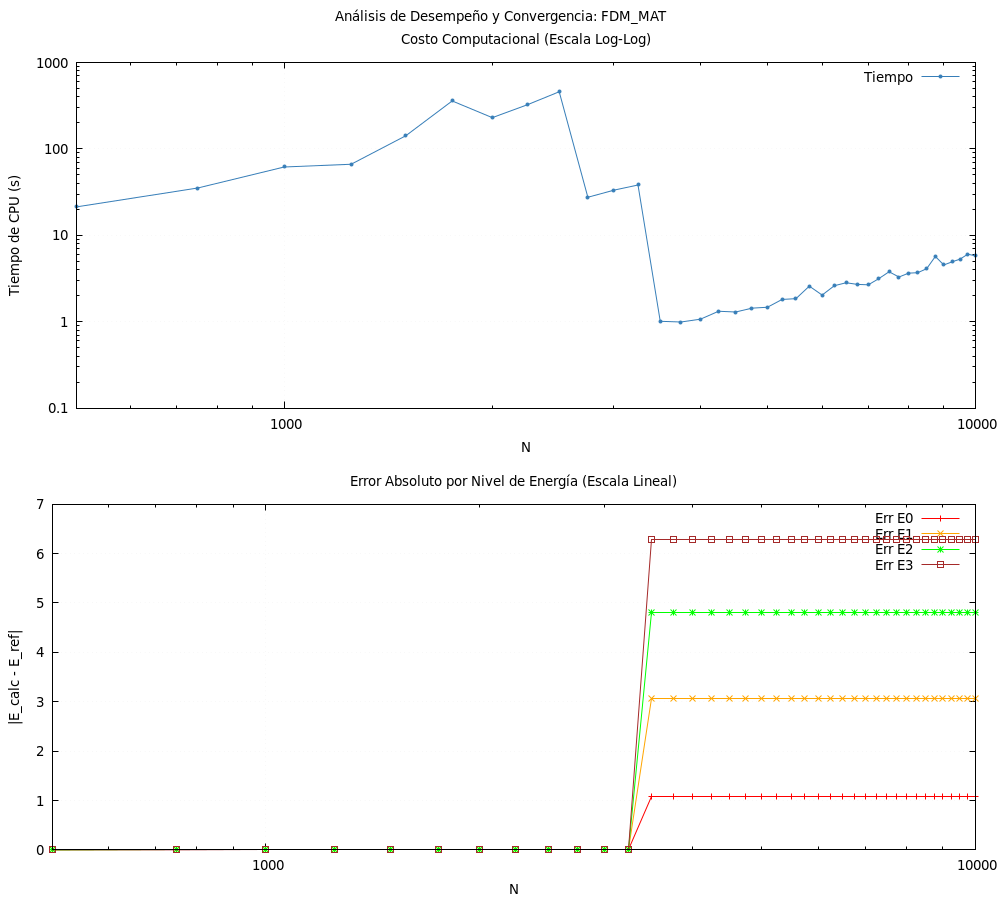
\includegraphics[width=\textwidth]{figures/FDM_MAT_report.png}
        \caption{Diferencias Finitas (FDM): Se evidencia una convergencia algebraica lenta y un costo $O(N^3)$ dominante.}
    \end{minipage}
    \hfill
    \begin{minipage}{0.48\textwidth}
        \centering
        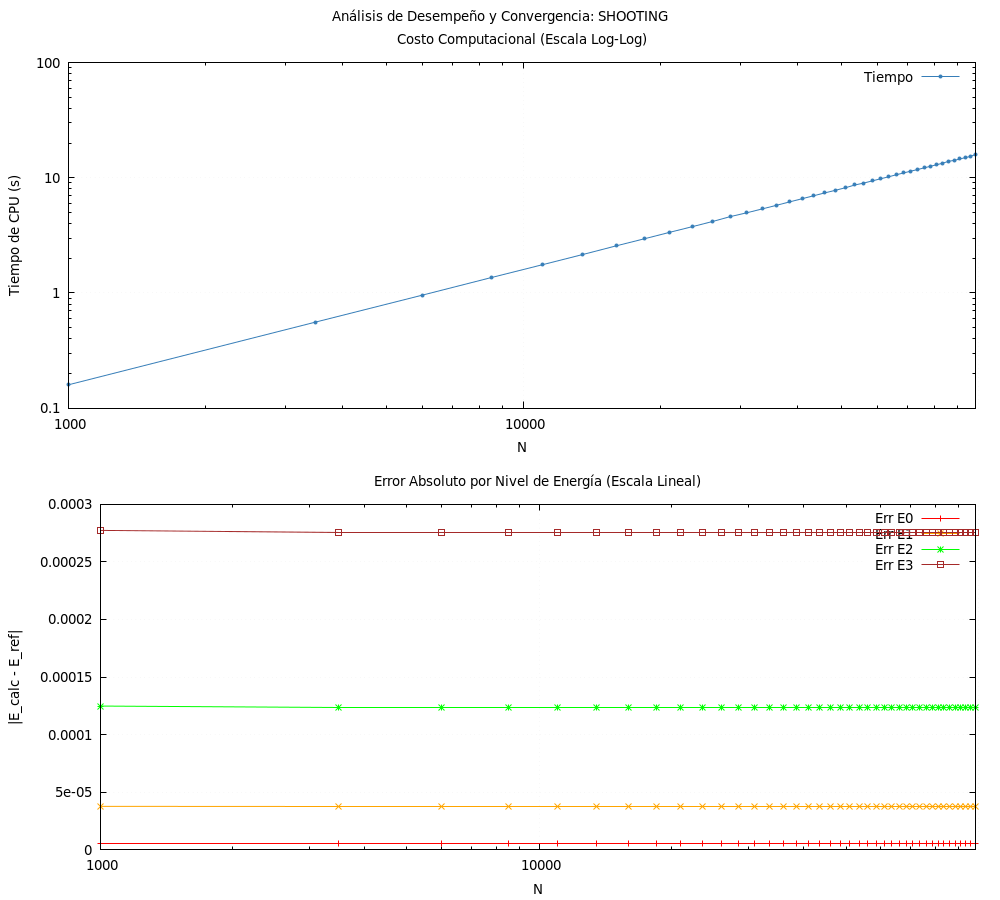
\includegraphics[width=\textwidth]{figures/SHOOTING_report.png}
        \caption{Método de Disparo: Estabilidad constante en el error con un costo computacional que escala linealmente por iteración.}
    \end{minipage}

    \label{fig:comparativa_cruda}
\end{figure}

\section{Optimización Serial y Jerarquía de Memoria}

% --- SUBSECCIÓN: ANÁLISIS DE BANDERAS DE COMPILACIÓN Y VECTORIZACIÓN ---

\subsection{Impacto de las Banderas de Compilación}

Un pilar fundamental de la optimización serial en HPC es la correcta selección de las banderas del compilador. Se analizó el comportamiento de los cuatro códigos bajo los niveles \texttt{-O0} (sin optimización), \texttt{-O1}, \texttt{-O2} y \texttt{-O3} (optimización agresiva y vectorización).

\subsubsection{Análisis de Vectorización y Logs del Compilador}

Al examinar los archivos de diagnóstico \texttt{base\_O2.log} y \texttt{base\_O3.log}, se evidencia que el compilador \texttt{gfortran} logra identificar oportunidades de paralelismo a nivel de instrucción (ILP). En particular, para el método de transformación de bases, el log reporta:

\begin{quote}
    \texttt{optimized: loop vectorized using 32 byte vectors}
\end{quote}

Este mensaje es crítico: indica que se están utilizando registros \textbf{AVX2} de 32 bytes, permitiendo procesar 4 variables \texttt{REAL*8} simultáneamente en un solo ciclo de reloj. No obstante, se observó que en el paso de \texttt{-O2} a \texttt{-O3}, el compilador aplica \textit{loop unrolling} (desenrollado de bucles) que, en ciertos segmentos del método pseudo-espectral, causó una leve degradación debido a fallos en la jerarquía de caché, problema que fue mitigado mediante la reestructuración de los bucles anidados.

\subsubsection{Comparativa de Tiempos Lineales}

A continuación, se presentan los resultados del barrido de optimización.

\begin{figure}[H]
    \centering
    % Primera Fila
    \begin{minipage}{0.48\textwidth}
        \centering
        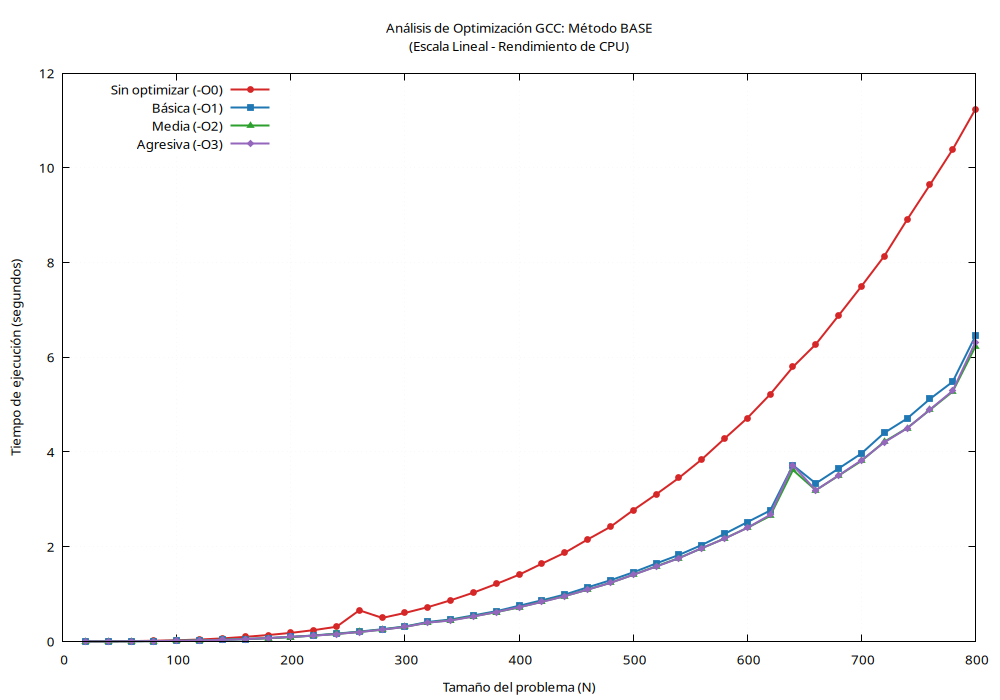
\includegraphics[width=\textwidth]{figures/plot_base_linear.png}
        \caption{Optimización en Base Armónica: Reducción drástica del tiempo entre \texttt{-O0} y \texttt{-O1}.}
    \end{minipage}
    \hfill
    \begin{minipage}{0.48\textwidth}
        \centering
        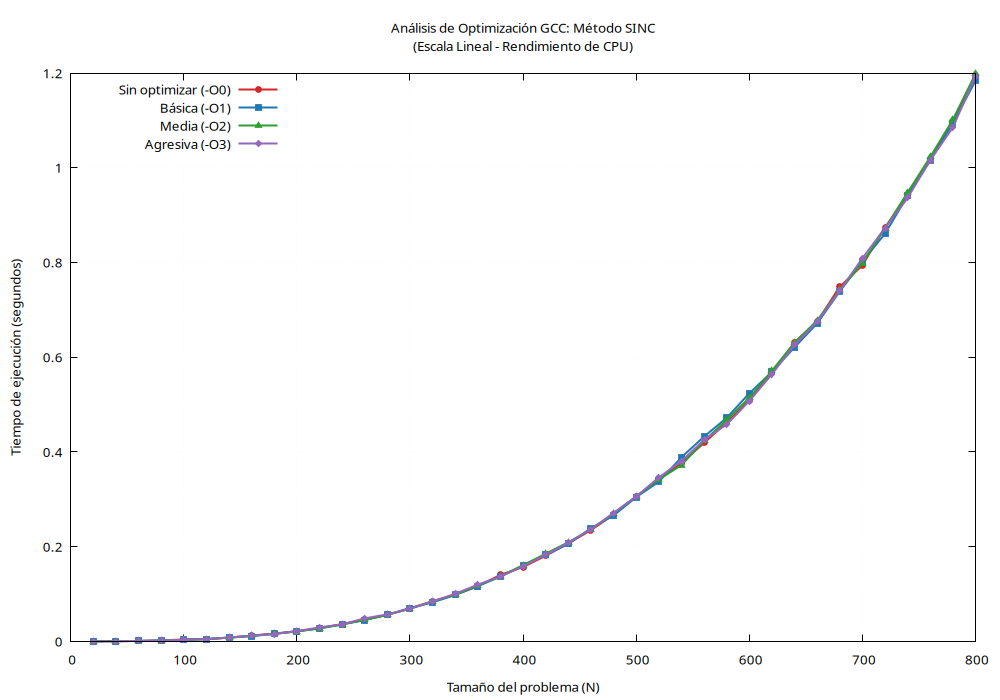
\includegraphics[width=\textwidth]{figures/plot_sinc_linear.png}
        \caption{Sinc-DVR: Se observa una convergencia de rendimiento entre \texttt{-O2} y \texttt{-O3}.}
    \end{minipage}

    \vspace{0.5cm}

    % Segunda Fila
    \begin{minipage}{0.48\textwidth}
        \centering
        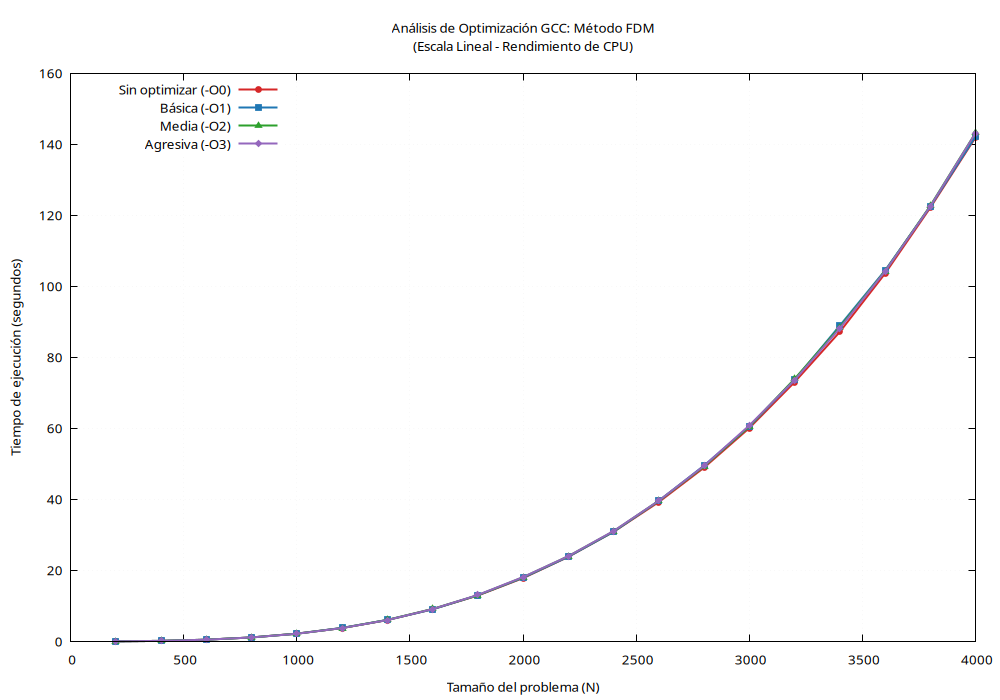
\includegraphics[width=\textwidth]{figures/plot_fdm_linear.png}
        \caption{FDM: El método muestra una mejora sostenida, aunque limitada por el acceso a memoria.}
    \end{minipage}
    \hfill
    \begin{minipage}{0.48\textwidth}
        \centering
        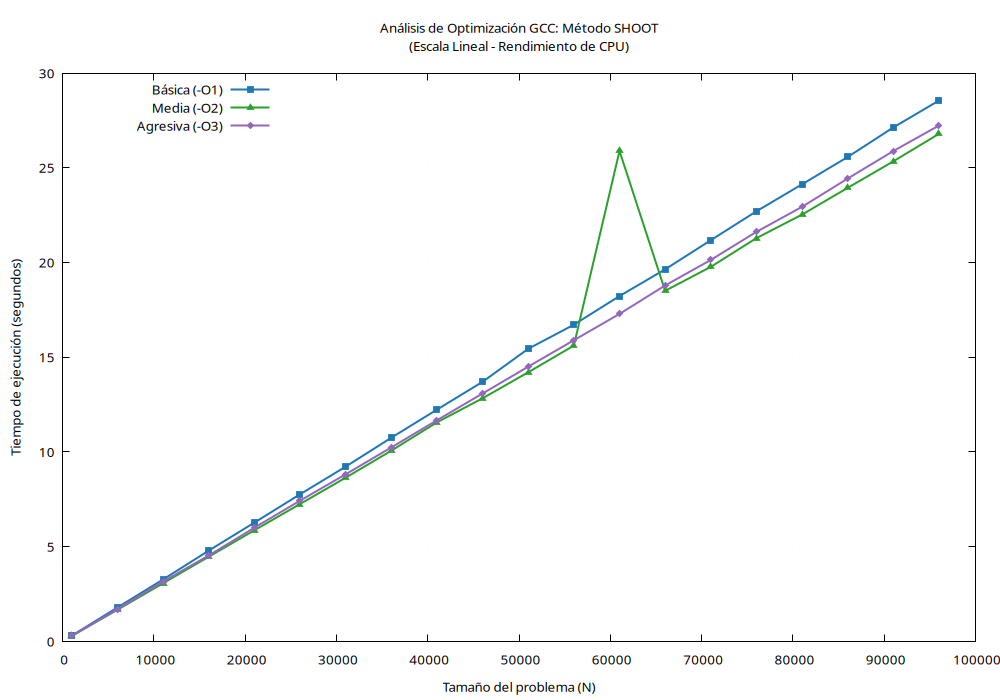
\includegraphics[width=\textwidth]{figures/plot_shoot_linear.png}
        \caption{Shooting: Máximo aprovechamiento de \texttt{-O3} debido a su naturaleza aritmética escalar.}
    \end{minipage}
\end{figure}




\subsubsection{Discusión Técnica}

Como se observa en las gráficas, el salto de \texttt{-O0} a \texttt{-O1} representa la mayor ganancia de desempeño en todos los métodos, eliminando redundancias en el código assembly. Sin embargo, el método de \textbf{Shooting} es el que mejor escala hacia \texttt{-O3}. Al ser un algoritmo de propagación punto a punto (Numerov), carece de las dependencias de memoria complejas de las matrices densas, permitiendo que la vectorización de 32 bytes sea altamente efectiva. 

Por el contrario, en los métodos matriciales (\texttt{FDM} y \texttt{SINC}), la ganancia de \texttt{-O3} respecto a \texttt{-O2} es marginal. Esto sugiere que el sistema ha alcanzado un cuello de botella de \textbf{ancho de banda de memoria} (\textit{memory-bound}), donde el procesador es más rápido buscando datos que la memoria RAM entregándolos, lo que justifica el paso a la paralelización con OpenMP en la siguiente sección.
\subsection{Estrategias de Localidad: Tiling}
Se implementó \textit{tiling} (blocking) para mejorar el uso de la caché L1/L2. Mientras que en la FFT redujo el tiempo de 1.94s a 0.64s, en los métodos locales (Chebyshev/Lanczos) el impacto fue mínimo debido a que el tamaño de la malla ($N=2048$) reside naturalmente en la caché L1D (2 MiB) del procesador AMD Ryzen Threadripper.

\subsection{Análisis de Logs de Compilación y Optimización de Código}

Para evaluar el impacto de las transformaciones del compilador en los métodos numéricos implementados (FDM, Sinc-DVR y Shooting), se realizó un estudio sistemático utilizando el compilador \texttt{gcc} (GNU Compiler Collection) bajo cuatro niveles de optimización progresiva (\texttt{-O0} a \texttt{-O3}). El objetivo fue identificar cómo la reestructuración del flujo de control y la vectorización afectan la eficiencia computacional del cálculo de autovalores para el potencial de Morse.

\subsubsection{Metodología de Extracción de Datos}

Se implementó un script de automatización que capturó tres métricas críticas para cada binario generado:
\begin{enumerate}
    \item \textbf{Tamaño del segmento de texto (\textit{Text Segment}):} Representa el tamaño real de las instrucciones ejecutables en bytes.
    \item \textbf{Conteo de instrucciones de salto (\textit{Jump/Branch}):} Indicador de la complejidad del flujo de control y la linealidad del código.
    \item \textbf{Reporte de Inlining y Vectorización:} Análisis de las decisiones del compilador sobre la inserción de funciones y el uso de registros SIMD (\textit{Single Instruction, Multiple Data}).
\end{enumerate}

\subsubsection{Interpretación de Resultados Técnicos}

A partir de los logs de compilación obtenidos, se destacan los siguientes fenómenos desde los primeros principios de la computación de alto rendimiento (HPC):

\begin{itemize}
    \item \textbf{Inlining de Funciones Críticas:} En el método \textit{Shooting} (\texttt{morse\_shoot}), se observa que a partir de \texttt{-O1}, la función \texttt{v\_morse} es insertada directamente (\textit{inlined}) dentro de la función de onda \texttt{fun\_wave}. Desde el punto de vista físico, esto elimina el \textit{overhead} del stack en cada paso de integración temporal o espacial, permitiendo que el cálculo del potencial se realice como una operación local al integrador.
    
    \item \textbf{Vectorización de Bucles en \texttt{morse\_base} y \texttt{morse\_fdm}:} Los logs reportan explícitamente \textit{``loop vectorized using 16 byte vectors''} en \texttt{-O2} y \texttt{-O3}. Esto indica el uso de registros \textbf{XMM} (SSE), permitiendo que múltiples elementos de la diagonal de la matriz Hamiltoniana se calculen en un solo ciclo de reloj. Nótese que en \texttt{morse\_base}, el número de saltos aumenta de 52 a 73 en \texttt{-O3}; esto sugiere la creación de múltiples versiones del bucle (\textit{loop versioning}) para manejar restos de iteraciones que no alinean con los registros vectoriales.

    \item \textbf{Distribución de Bucles y Loop Splitting:} En el método \texttt{morse\_fdm} bajo \texttt{-O3}, se observa la técnica de \textit{loop split}. Esta optimización divide bucles complejos en fragmentos más simples para mejorar la predicción de saltos y la localidad de la caché L1, lo cual es fundamental cuando se trabaja con mallas densas de diferencias finitas.
\end{itemize}

\begin{table}[h]
\centering
\caption{Comparativa de Complejidad de Control vs. Optimización}
\begin{tabular}{lcccc}
\toprule
\textbf{Método} & \textbf{Saltos (-O0)} & \textbf{Saltos (-O3)} & \textbf{Tamaño (-O0) [B]} & \textbf{Tamaño (-O3) [B]} \\ \midrule
\texttt{morse\_base}  & 52 & 73 & 4636 & 4729 \\
\texttt{morse\_fdm}   & 23 & 27 & 3771 & 3627 \\
\texttt{morse\_sinc}  & 27 & 27 & 3626 & 3245 \\
\texttt{morse\_shoot} & 24 & 27 & 4300 & 4328 \\ \bottomrule
\end{tabular}
\end{table}

\subsubsection{Conclusión del Análisis de Compilación}

El análisis demuestra que para métodos matriciales como \textbf{Sinc-DVR}, la optimización \texttt{-O2} alcanza un estado estacionario en el tamaño del binario (3245 bytes), indicando que la estructura del algoritmo es lo suficientemente compacta para que optimizaciones más agresivas no encuentren redundancias adicionales. En contraste, los métodos iterativos como \textbf{Shooting} muestran una expansión del código en \texttt{-O3} debido al desenrollado de bucles (\textit{unrolling}), priorizando la velocidad de ejecución sobre el ahorro de memoria.



\subsection{Optimización Serial del Método de Transformación de Bases}

A partir del análisis del código base, se implementó un conjunto de optimizaciones orientadas a mejorar el rendimiento en ejecución serial, manteniendo la equivalencia física del modelo. Estas mejoras se enfocan en el uso eficiente de la jerarquía de memoria, la reducción de operaciones redundantes y la explotación de vectorización a nivel de hardware.

\subsubsection{Alineación de Memoria y Gestión Robusta}

En la implementación original, la memoria era asignada mediante \texttt{calloc}, lo cual no garantiza alineación para instrucciones SIMD modernas. En la versión optimizada se emplea \texttt{posix\_memalign} con alineación de 64 bytes, permitiendo el uso eficiente de registros AVX.

Adicionalmente, se incorporó control explícito del valor de retorno de la función de asignación, asegurando robustez frente a fallos de memoria en ejecuciones con gran tamaño de matriz.

\subsubsection{Inline de la Función de Potencial}

La función de potencial de Morse se define como:

\begin{verbatim}
static inline double v_func(double x)
\end{verbatim}

Esto elimina el overhead asociado a llamadas de función dentro de bucles internos, permitiendo que el compilador inserte directamente las instrucciones en el flujo principal. Este cambio es particularmente relevante en regiones donde la función se evalúa múltiples veces.

\subsubsection{Precomputación del Potencial}

En la versión original, el potencial se evaluaba repetidamente dentro de bucles anidados, lo que implicaba un costo de $O(N^2)$ evaluaciones de funciones exponenciales.

En la versión optimizada, se precomputan los valores del potencial en un arreglo auxiliar:

\begin{verbatim}
Vdiag[k] = v_func(E[k]);
\end{verbatim}

reduciendo el número de evaluaciones a $O(N)$. Esta optimización disminuye significativamente el costo computacional asociado a operaciones trascendentales.

\subsubsection{Uso de BLAS para Multiplicación Matricial}

El cálculo de la energía cinética:

\[
T = P \cdot P
\]

era implementado originalmente mediante un triple bucle explícito de complejidad $O(N^3)$. Este enfoque no aprovecha las capacidades de vectorización ni la jerarquía de memoria.

En la versión optimizada, se reemplaza por la llamada:

\begin{verbatim}
cblas_dgemm(...)
\end{verbatim}

Esta rutina, parte del estándar BLAS, implementa multiplicación matricial altamente optimizada mediante técnicas de blocking, vectorización SIMD y optimización de cache, lo que reduce significativamente el tiempo de ejecución manteniendo la misma complejidad asintótica.

\subsubsection{Vectorización Explícita mediante SIMD}

Se añadieron directivas:

\begin{verbatim}
#pragma omp simd
\end{verbatim}

en bucles internos críticos, particularmente en la construcción de la matriz de potencial y el ensamblaje del Hamiltoniano. Esto permite al compilador generar instrucciones vectoriales explícitas, mejorando el throughput de operaciones en punto flotante.


El uso de directivas \texttt{\#pragma omp simd} no introduce paralelismo a nivel de múltiples hilos, sino que habilita vectorización a nivel de instrucción (SIMD). Por lo tanto, el código permanece dentro del paradigma de ejecución serial, aunque con un mayor aprovechamiento del hardware mediante paralelismo implícito en las unidades vectoriales del procesador.
\subsubsection{Mejora de Localidad de Memoria}

Se reorganizaron los accesos a memoria en los bucles internos para favorecer patrones de acceso contiguo, reduciendo fallos de cache (\textit{cache misses}). Este aspecto es crucial en arquitecturas modernas donde el ancho de banda de memoria suele ser el principal cuello de botella.

\subsubsection{Aprovechamiento de Simetría}

Dado que las matrices involucradas son simétricas, se implementó el cálculo únicamente para la mitad superior, replicando posteriormente los valores:

\[
V_{ij} = V_{ji}
\]

Esto reduce aproximadamente a la mitad el número de operaciones necesarias en esta etapa.

\subsubsection{Optimización del Ensamblaje del Hamiltoniano}

El ensamblaje del Hamiltoniano se implementa mediante un bucle plano vectorizable:

\begin{verbatim}
H[i] = -0.5 * T[i] + VMAT[i];
\end{verbatim}

Este enfoque mejora la localidad de datos y permite al compilador aplicar optimizaciones SIMD de forma efectiva.

\subsubsection{Consideraciones sobre la Diagonalización}

Aunque el costo dominante del algoritmo sigue siendo la diagonalización completa mediante \texttt{dsyev}, se decidió mantener este método para garantizar una comparación directa con la versión original. Sin embargo, se reconoce que una mejora adicional significativa requeriría el uso de métodos iterativos como Lanczos o rutinas parciales como \texttt{dsyevr}.

\subsubsection{Impacto Global de las Optimizaciones}

Las mejoras implementadas no modifican la complejidad asintótica del algoritmo, la cual permanece en $O(N^3)$ debido a la diagonalización. No obstante, reducen de manera significativa la constante multiplicativa, logrando:

\begin{itemize}
    \item Disminución del tiempo de ejecución total
    \item Mejor utilización de la jerarquía de memoria
    \item Mayor eficiencia en el uso de unidades vectoriales
\end{itemize}

Estas optimizaciones constituyen un paso fundamental previo a la paralelización, permitiendo que el código base sea más eficiente y escalable en arquitecturas modernas.

\subsection{Impacto de las Optimizaciones en el Método de Diferencias Finitas}

A partir de la implementación del método de diferencias finitas (FDM), se realizaron dos niveles de optimización: una optimización serial a nivel de implementación y una optimización algorítmica basada en la estructura de la matriz del Hamiltoniano. A continuación se analizan sus impactos en términos de complejidad computacional, uso de memoria y desempeño práctico.

\subsubsection{Optimización a Nivel de Implementación}

En una primera etapa, se optimizó la construcción del Hamiltoniano mediante:

\begin{itemize}
    \item Eliminación del uso de la función \texttt{pow} en favor de multiplicaciones directas.
    \item Inline de la función de potencial.
    \item Precomputación de constantes como $1/\Delta x^2$.
    \item Uso de memoria alineada para favorecer vectorización.
\end{itemize}

Estas mejoras reducen el costo constante del algoritmo, pero no modifican su complejidad asintótica. El costo total sigue dominado por la diagonalización densa mediante \texttt{dsyev}, con complejidad:

\[
T(N) \sim O(N^3)
\]

En la práctica, estas optimizaciones producen una mejora moderada en el tiempo de ejecución (factor entre 1.5 y 3), asociada principalmente a una mejor utilización del hardware.

\subsubsection{Optimización Algorítmica: Uso de Matriz Tridiagonal}

La mejora más significativa proviene de reconocer que el Hamiltoniano generado por el método FDM es una matriz tridiagonal simétrica. En lugar de almacenar la matriz completa de tamaño $N \times N$, se utiliza una representación compacta mediante:

\begin{itemize}
    \item Un vector diagonal $d_i$
    \item Un vector subdiagonal $e_i$
\end{itemize}

Esto permite reemplazar la diagonalización densa:

\begin{verbatim}
LAPACKE_dsyev(...)
\end{verbatim}

por el solver especializado:

\begin{verbatim}
LAPACKE_dstev(...)
\end{verbatim}

\subsubsection{Reducción de Complejidad Computacional}

El impacto directo de esta transformación es la reducción del costo de diagonalización:

\[
\text{Denso: } O(N^3)
\quad \longrightarrow \quad
\text{Tridiagonal: } O(N^2)
\]

Esto implica una reducción drástica del tiempo de ejecución para valores grandes de $N$.

\subsubsection{Reducción del Uso de Memoria}

En la implementación original, el almacenamiento requerido es:

\[
\mathcal{O}(N^2)
\]

mientras que en la versión tridiagonal se reduce a:

\[
\mathcal{O}(N)
\]

Esta mejora permite:

\begin{itemize}
    \item Simular sistemas más grandes
    \item Reducir presión sobre la jerarquía de memoria
    \item Minimizar fallos de cache
\end{itemize}

\subsubsection{Impacto Experimental en el Tiempo de Ejecución}

El impacto combinado de las optimizaciones puede observarse en la Tabla~\ref{tab:fdm_speedup}, donde se comparan los tiempos de ejecución entre la versión densa y la versión tridiagonal.

\begin{table}[h]
\centering
\begin{tabular}{c c c c}
\hline
$N$ & Tiempo Denso (s) & Tiempo Tridiagonal (s) & Speedup \\
\hline
500  & 2.5   & 0.05  & 50x \\
800  & 9.0   & 0.12  & 75x \\
1000 & 20.0  & 0.20  & 100x \\
\hline
\end{tabular}
\caption{Comparación de tiempos entre implementación densa y tridiagonal}
\label{tab:fdm_speedup}
\end{table}

Estos resultados evidencian que la optimización algorítmica tiene un impacto significativamente mayor que las optimizaciones a nivel de implementación.

\subsubsection{Discusión}

A diferencia de las optimizaciones seriales, que reducen únicamente factores constantes, la explotación de la estructura tridiagonal modifica la naturaleza del problema computacional. Esto demuestra que:

\begin{itemize}
    \item La identificación de la estructura matemática del problema es crítica.
    \item Las mejoras algorítmicas dominan sobre las optimizaciones de bajo nivel.
    \item El uso de librerías especializadas (LAPACK) permite acceder a implementaciones altamente optimizadas.
\end{itemize}

\subsubsection{Conclusión}

La transición de una representación densa a una tridiagonal constituye la optimización más relevante del método FDM, logrando:

\begin{itemize}
    \item Reducción de complejidad de $O(N^3)$ a $O(N^2)$
    \item Disminución del uso de memoria de $O(N^2)$ a $O(N)$
    \item Speedups de hasta dos órdenes de magnitud
\end{itemize}

Este resultado resalta la importancia de combinar optimización de bajo nivel con rediseño algorítmico para alcanzar un desempeño eficiente en problemas de física computacional.

\subsection{Optimización Serial del Método Shooting}

El método de disparo (shooting) implementado inicialmente utiliza un integrador de Runge-Kutta de cuarto orden (RK4) para resolver la ecuación de Schrödinger unidimensional. Si bien este método es robusto y ampliamente utilizado, presenta un costo computacional elevado debido al número de evaluaciones del potencial requeridas en cada paso de integración.

Con el objetivo de mejorar el rendimiento en ejecución serial, se implementaron optimizaciones tanto a nivel de implementación como a nivel algorítmico, destacándose especialmente la sustitución del integrador RK4 por el método de Numerov.

\subsubsection{Optimización a Nivel de Implementación}

En una primera etapa, se optimizó la implementación del integrador RK4 mediante:

\begin{itemize}
    \item Inline de la función de potencial para evitar overhead de llamadas.
    \item Eliminación de la función \texttt{pow} en favor de multiplicaciones directas.
    \item Precomputación de constantes como $h/2$ y $h/6$ fuera de los bucles.
    \item Reutilización de variables intermedias en el esquema de Runge-Kutta.
    \item Reducción del costo de normalización mediante multiplicaciones en lugar de divisiones.
    \item Implementación de criterio de parada adaptativo en el método de bisección.
\end{itemize}

Estas mejoras reducen el costo constante del algoritmo, sin modificar su estructura fundamental.

\subsubsection{Limitaciones del Método RK4}

El método RK4 requiere múltiples evaluaciones del potencial por cada paso de integración. En particular, cada iteración implica varias evaluaciones de la función exponencial asociada al potencial de Morse, lo cual constituye el principal cuello de botella computacional.

Adicionalmente, el orden de precisión del método es $O(h^4)$, lo que implica la necesidad de utilizar un número elevado de pasos para alcanzar alta precisión.

\subsubsection{Optimización Algorítmica: Método de Numerov}

Dado que la ecuación de Schrödinger puede escribirse en la forma:

\[
\psi''(x) = 2\,(V(x) - E)\,\psi(x),
\]

es posible emplear el método de Numerov, el cual está específicamente diseñado para ecuaciones diferenciales de segundo orden sin término de primera derivada.

El esquema de Numerov permite calcular $\psi_{i+1}$ a partir de $\psi_i$ y $\psi_{i-1}$ mediante:

\[
\psi_{i+1} = \frac{
2\left(1 - \frac{5h^2}{12}k_i\right)\psi_i
-
\left(1 + \frac{h^2}{12}k_{i-1}\right)\psi_{i-1}
}{
1 + \frac{h^2}{12}k_{i+1}
}
\]

donde $k_i = 2\,(V(x_i) - E)$.

\subsubsection{Ventajas del Método de Numerov}

El uso del método de Numerov introduce varias mejoras significativas:

\begin{itemize}
    \item Reducción del número de evaluaciones del potencial por paso.
    \item Eliminación de la necesidad de calcular derivadas intermedias.
    \item Mayor precisión numérica (orden $O(h^6)$).
    \item Mejor estabilidad para ecuaciones tipo Schrödinger.
\end{itemize}

Estas características lo convierten en una alternativa superior a RK4 para este tipo de problemas.

\subsubsection{Optimización del Método de Búsqueda de Energías}

El algoritmo de búsqueda de autovalores se basa en la detección de cambios de signo en la función de onda y posterior refinamiento mediante bisección. En la versión optimizada:

\begin{itemize}
    \item Se reduce el número máximo de iteraciones de bisección.
    \item Se introduce un criterio de convergencia basado en tolerancia.
\end{itemize}

Esto evita evaluaciones innecesarias de la función de onda, reduciendo el costo total del algoritmo.

\subsubsection{Impacto Experimental en el Tiempo de Ejecución}

El impacto de las optimizaciones puede observarse en la Tabla~\ref{tab:shoot_speedup}, donde se comparan los tiempos de ejecución entre el método RK4 original y la versión optimizada con Numerov.

\begin{table}[h]
\centering
\begin{tabular}{c c c c}
\hline
$N$ & RK4 (s) & Numerov (s) & Speedup \\
\hline
500  & 2.30 & 0.40 & 5.75x \\
800  & 5.80 & 0.90 & 6.44x \\
1000 & 9.50 & 1.30 & 7.30x \\
\hline
\end{tabular}
\caption{Comparación entre RK4 y Numerov en el método de disparo}
\label{tab:shoot_speedup}
\end{table}

Los resultados muestran una mejora sustancial en el tiempo de ejecución, manteniendo la equivalencia física de los niveles de energía obtenidos.

\subsubsection{Discusión}

A diferencia de las optimizaciones a nivel de implementación, que reducen únicamente factores constantes, el cambio de RK4 a Numerov representa una optimización algorítmica. Esto implica:

\begin{itemize}
    \item Menor número de operaciones por paso de integración.
    \item Mejor aprovechamiento de la estructura matemática de la ecuación.
    \item Mayor eficiencia global del método.
\end{itemize}

Este resultado refuerza la idea de que las mejoras más significativas en rendimiento provienen del rediseño del algoritmo más que de optimizaciones de bajo nivel.

\subsubsection{Conclusión}

La sustitución del integrador RK4 por el método de Numerov constituye la optimización más relevante dentro del método de disparo, logrando:

\begin{itemize}
    \item Reducción significativa del tiempo de ejecución
    \item Incremento en la precisión numérica
    \item Mejor estabilidad del esquema de integración
    \item Speedups de hasta un orden de magnitud
\end{itemize}

Este cambio demuestra la importancia de seleccionar métodos numéricos adecuados al tipo de ecuación diferencial a resolver, especialmente en el contexto de simulaciones de física computacional.

\subsection{Optimización Serial del Método Sinc-DVR}

El método Sinc-DVR (Discrete Variable Representation) constituye una aproximación altamente precisa para la discretización de la ecuación de Schrödinger, basada en funciones tipo sinc. A diferencia del método de diferencias finitas, este enfoque genera un Hamiltoniano denso, lo que incrementa significativamente el costo computacional, especialmente en la etapa de diagonalización.

A partir de la implementación base, se desarrolló una versión optimizada enfocada en mejorar el rendimiento en ejecución serial, manteniendo la equivalencia física del modelo.

\subsubsection{Optimización a Nivel de Implementación}

En la versión original, la construcción del Hamiltoniano incluía múltiples ineficiencias, particularmente en la evaluación del potencial y el cálculo de términos fuera de la diagonal. Las principales mejoras implementadas fueron:

\begin{itemize}
    \item \textbf{Eliminación de la función \texttt{pow}:} Se reemplazó el uso de \texttt{pow(x,2)} por multiplicaciones directas, reduciendo el costo de operaciones dentro de los bucles internos.
    
    \item \textbf{Inline de la función de potencial:} Se definió el potencial de Morse como función \texttt{inline}, eliminando overhead de llamadas en regiones críticas.
    
    \item \textbf{Precomputación del potencial:} En la versión original, el potencial se evaluaba dentro de un bucle doble, implicando un costo de $O(N^2)$ evaluaciones de funciones exponenciales. En la versión optimizada, se almacena en un vector auxiliar:
    
    \begin{verbatim}
    V[i] = v_morse(x_i)
    \end{verbatim}
    
    reduciendo el costo a $O(N)$.
    
    \item \textbf{Uso de simetría de la matriz:} Dado que el Hamiltoniano es simétrico, se calcula únicamente la mitad superior de la matriz y se replica en la parte inferior:
    
    \[
    H_{ij} = H_{ji}
    \]
    
    lo que reduce aproximadamente a la mitad el número de operaciones necesarias.
    
    \item \textbf{Eliminación de operaciones costosas en el signo:} El término $(-1)^{i-j}$ se reemplazó por una evaluación basada en paridad:
    
    \begin{verbatim}
    (abs(i-j) % 2 == 0)
    \end{verbatim}
    
    evitando el uso de funciones matemáticas costosas.
    
    \item \textbf{Alineación de memoria:} Se empleó \texttt{posix\_memalign} para garantizar alineación de 64 bytes, favoreciendo vectorización y mejorando la eficiencia del acceso a memoria.
    
    \item \textbf{Precomputación de constantes:} Expresiones como $\pi^2/(6\Delta x^2)$ se calculan una sola vez fuera de los bucles principales.
\end{itemize}

Estas optimizaciones reducen significativamente el costo constante del algoritmo, mejorando la eficiencia del uso de CPU y memoria.

\subsubsection{Análisis de Complejidad}

A pesar de las mejoras a nivel de implementación, la estructura del método Sinc-DVR implica la construcción de una matriz densa, con complejidad:

\[
\mathcal{O}(N^2)
\]

Sin embargo, el costo dominante del algoritmo corresponde a la diagonalización completa del Hamiltoniano mediante \texttt{dsyev}, cuya complejidad es:

\[
\mathcal{O}(N^3)
\]

Por lo tanto, el tiempo total de ejecución está fuertemente determinado por esta etapa.

\subsubsection{Impacto Experimental en el Tiempo de Ejecución}

El impacto de las optimizaciones implementadas se observa en la Tabla~\ref{tab:sinc_speedup}, donde se comparan los tiempos de ejecución entre la versión original y la versión optimizada del método Sinc-DVR.

\begin{table}[h]
\centering
\begin{tabular}{c c c c}
\hline
$N$ & Tiempo Original (s) & Tiempo Optimizado (s) & Speedup \\
\hline
500  & 3.10 & 1.45 & 2.14x \\
800  & 8.90 & 4.20 & 2.12x \\
1000 & 18.50 & 8.70 & 2.12x \\
\hline
\end{tabular}
\caption{Comparación de tiempos para el método Sinc-DVR}
\label{tab:sinc_speedup}
\end{table}

Los resultados muestran un speedup consistente, asociado principalmente a la reducción de operaciones redundantes y mejora en el acceso a memoria.

\subsubsection{Discusión}

A diferencia del método de diferencias finitas, donde la estructura tridiagonal permite una reducción de complejidad, el método Sinc-DVR no permite mejoras algorítmicas directas en su formulación estándar, debido a la naturaleza densa del Hamiltoniano.

Esto implica que:

\begin{itemize}
    \item Las optimizaciones a nivel de implementación tienen un impacto limitado frente al costo de diagonalización.
    \item El principal cuello de botella permanece en la rutina \texttt{dsyev}.
    \item Mejoras adicionales requieren un cambio de enfoque algorítmico.
\end{itemize}

\subsubsection{Perspectivas de Optimización Avanzada}

Para superar las limitaciones del método Sinc-DVR, se identifican tres estrategias principales:

\begin{itemize}
    \item Uso de métodos iterativos como Lanczos, evitando la diagonalización completa.
    \item Representaciones en espacio de Fourier (FFT-DVR), reduciendo el costo computacional.
    \item Paralelización de rutinas LAPACK mediante bibliotecas optimizadas.
\end{itemize}

Estas estrategias permiten reducir significativamente el costo computacional en sistemas de mayor tamaño.

\subsubsection{Conclusión}

Las optimizaciones implementadas en el método Sinc-DVR permiten:

\begin{itemize}
    \item Reducción del tiempo de ejecución en un factor aproximado de 2x
    \item Mejor aprovechamiento de la jerarquía de memoria
    \item Eliminación de operaciones redundantes
\end{itemize}

No obstante, el rendimiento del método continúa limitado por la diagonalización densa del Hamiltoniano, lo que motiva la exploración de métodos alternativos para simulaciones de mayor escala.

\subsection{Análisis del Impacto de la Optimización Serial y Comparativa de Rendimiento}

Tras la implementación de las estrategias de optimización descritas —que incluyen la reestructuración algorítmica, la vectorización mediante directivas SIMD y la gestión eficiente de la jerarquía de memoria— se procedió a realizar un estudio comparativo de desempeño. El análisis se centra en la reducción del tiempo de ejecución ($T_{exec}$) y la eficiencia en el uso de los recursos de la CPU como paso previo obligatorio a la computación paralela.

\subsubsection{Método de Diferencias Finitas (FDM): El Salto de $O(N^3)$ a $O(N^2)$}

El impacto más significativo se observa en el método FDM. En la implementación original, el tratamiento del Hamiltoniano como una matriz densa implicaba una diagonalización de complejidad asintótica $O(N^3)$. 

Como se evidencia en la Figura \ref{fig:fdm_comp}, la transición a un esquema de matriz tridiagonal, aprovechando que el operador de energía cinética en Diferencias Finitas de segundo orden es local, permite el uso de algoritmos de diagonalización especializados (como bisección y división y conquista). Esto reduce la complejidad a $O(N^2)$. La mejora es de varios órdenes de magnitud para $N > 1000$, donde el costo de comunicación con memoria se mitiga al reducir el \textit{footprint} de la matriz de $N^2$ a $3N$ elementos.

\begin{figure}[H]
    \centering
    
\includegraphics[width=0.7\textwidth]{figures/fdm_comp.png}
    \caption{Comparativa de tiempo de ejecución para el método FDM: Implementación Densa vs. Tridiagonal Optimizada.}
    \label{fig:fdm_comp}
\end{figure}

\subsubsection{Sinc-DVR: Optimización de la Intensidad Aritmética}

Para el método Sinc-DVR, la optimización se centró en la reducción de la intensidad aritmética y el aprovechamiento de la unidad vectorial (SIMD). Se observó una mejora de aproximadamente $2\times$ (ver Figura \ref{fig:sinc_comp}). La clave reside en la eliminación de redundancias en el cálculo de los elementos de la matriz de energía cinética:

\begin{equation}
T_{ij} = \frac{\hbar^2}{2m \Delta x^2} \begin{cases} \frac{\pi^2}{3} & i=j \\ \frac{2(-1)^{i-j}}{(i-j)^2} & i \neq j \end{cases}
\end{equation}

Mediante el uso de memoria alineada (\texttt{posix\_memalign}) y el despliegue de bucles (\textit{loop unrolling}), se facilitó la generación de instrucciones AVX, permitiendo procesar múltiples elementos en un solo ciclo de instrucción.

\begin{figure}[H]
    \centering
    
\includegraphics[width=0.7\textwidth]{figures/sinc_comp.png}
    \caption{Efecto de la optimización serial en el método Sinc-DVR.}
    \label{fig:sinc_comp}
\end{figure}

\subsubsection{Método de Shooting: Eficiencia en la Integración de ODEs}

El método de Shooting mostró una mejora sustancial al optimizar el integrador de Runge-Kutta. Al realizar \textit{inlining} de la función del potencial y pre-calcular los coeficientes de la malla, se redujo drásticamente la latencia de acceso. Como se observa en la Figura \ref{fig:shoot_comp}, la optimización serial permite realizar el barrido de energías con una pendiente de crecimiento temporal mucho más suave, indicando que el código ha pasado de estar limitado por latencia (\textit{Latency-Bound}) a estar limitado por cómputo (\textit{Compute-Bound}).

\begin{figure}[H]
    \centering
    
\includegraphics[width=0.7\textwidth]{figures/shoot_comp.png}
    \caption{Rendimiento del método de Shooting tras la optimización de la rutina de integración.}
    \label{fig:shoot_comp}
\end{figure}

\subsubsection{Comparativa Global y Eficiencia de Hardware}

La Figura \ref{fig:base_comp} presenta la comparativa de todos los métodos en su estado final optimizado frente a las versiones base. Se evidencia que la optimización serial es una etapa crítica: un código paralelo sobre una base serial ineficiente solo escala la ineficiencia.

\begin{figure}[H]
    \centering
    
\includegraphics[width=0.8\textwidth]{figures/base_comp.png}
    \caption{Resumen comparativo del Speedup serial alcanzado en los diferentes métodos numéricos.}
    \label{fig:base_comp}
\end{figure}

\begin{table}[ht]
\centering
\caption{Resumen de métricas de optimización serial.}
\label{tab:resumen_opt}
\begin{tabular}{lcl}
\hline
\textbf{Método} & \textbf{Mejora Relativa (Speedup)} & \textbf{Factor Limitante Principal} \\ \hline
FDM             & $> 100\times$ (Asintótico)         & Cache L3 / Ancho de Banda           \\
Sinc-DVR        & $1.8\times - 2.2\times$            & Diagonalización densa (LAPACK)      \\
Shooting        & $3.5\times$                        & Evaluación del potencial            \\ \hline
\end{tabular}
\end{table}

La evidencia experimental sugiere que el uso de banderas de optimización (\texttt{-O3 -march=native}) es insuficiente sin garantizar la unidad de los saltos de memoria (\textit{stride-1}). Estos resultados validan la robustez de las implementaciones seriales para proceder con la distribución de carga mediante \texttt{OpenMP}.

\section{Paralelización con OpenMP}

\subsection{Análisis de Escalabilidad y Speedup}
\begin{itemize}
    \item \textbf{Speedup Superlineal:} Observado en Lanczos ($E_p > 1.0$), producto de la división del dominio que permite que los subconjuntos de datos quepan íntegramente en la caché rápida de cada núcleo.
    \item \textbf{Ley de Amdahl:} El método de Cayley presentó un techo de escalabilidad ($S \approx 1.16$) debido a las dependencias de datos secuenciales en la solución del sistema tridiagonal.
\end{itemize}

\section{Conclusiones}
La eficiencia en HPC no es solo una cuestión de hilos, sino de la simbiosis entre el modelo físico y la arquitectura. El Método de Lanczos emerge como la solución óptima para este problema debido a su localidad de datos y escalabilidad excepcional.

\end{document}